\newif\ifshowsolutions
\showsolutionstrue
\documentclass{article}
\usepackage{listings}
\usepackage{amsmath}
%\usepackage{subfigure}
\usepackage{subfig}
\usepackage{amsthm}
\usepackage{amsmath}
\usepackage{amssymb}
\usepackage{graphicx}
\usepackage{mdwlist}
\usepackage[colorlinks=true]{hyperref}
\usepackage{geometry}
\usepackage{titlesec}
\geometry{margin=1in}
\geometry{headheight=2in}
\geometry{top=2in}
\usepackage{palatino}
\usepackage{mathrsfs}
\usepackage{fancyhdr}
\usepackage{paralist}
\usepackage{todonotes}
\setlength{\marginparwidth}{2.15cm}
\usepackage{tikz}
\usetikzlibrary{positioning,shapes,backgrounds}
\usepackage{float} % Place figures where you ACTUALLY want it
\usepackage{comment} % a hack to toggle sections
\usepackage{ifthen}
\usepackage{mdframed}
\usepackage{verbatim}
\usepackage[strings]{underscore}
\usepackage{listings}
\usepackage{bbm}
\rhead{}
\lhead{}

\renewcommand{\baselinestretch}{1.15}

% Shortcuts for commonly used operators
\newcommand{\E}{\mathbb{E}}
\newcommand{\Var}{\operatorname{Var}}
\newcommand{\Cov}{\operatorname{Cov}}
\newcommand{\Bias}{\operatorname{Bias}}
\DeclareMathOperator{\argmin}{arg\,min}
\DeclareMathOperator{\argmax}{arg\,max}

% do not number subsection and below
\setcounter{secnumdepth}{1}

% custom format subsection
\titleformat*{\subsection}{\large\bfseries}

% set up the \question shortcut
\newcounter{question}[section]
\newenvironment{question}[1][]
  {\refstepcounter{question}\par\addvspace{1em}\textbf{Question~\Alph{question}\!
    \ifthenelse{\equal{#1}{}}{}{ [#1 points]}: }}
    {\par\vspace{\baselineskip}}

\newcounter{subquestion}[question]
\newenvironment{subquestion}[1][]
  {\refstepcounter{subquestion}\par\medskip\textbf{\roman{subquestion}.\!
    \ifthenelse{\equal{#1}{}}{}{ [#1 points]:}} }
  {\par\addvspace{\baselineskip}}

\titlespacing\section{0pt}{12pt plus 2pt minus 2pt}{0pt plus 2pt minus 2pt}
\titlespacing\subsection{0pt}{12pt plus 4pt minus 2pt}{0pt plus 2pt minus 2pt}
\titlespacing\subsubsection{0pt}{12pt plus 4pt minus 2pt}{0pt plus 2pt minus 2pt}


\newenvironment{hint}[1][]
  {\begin{em}\textbf{Hint: }}{\end{em}}

\ifshowsolutions
  \newenvironment{solution}[1][]
    {\par\medskip \begin{mdframed}\textbf{Solution~\Alph{question}#1:} \begin{em}}
    {\end{em}\medskip\end{mdframed}\medskip}
  \newenvironment{subsolution}[1][]
    {\par\medskip \begin{mdframed}\textbf{Solution~\Alph{question}#1.\roman{subquestion}:} \begin{em}}
    {\end{em}\medskip\end{mdframed}\medskip}
\else
  \excludecomment{solution}
  \excludecomment{subsolution}
\fi

\newcommand{\boldline}[1]{\underline{\textbf{#1}}}

\chead{%
  {\vbox{%
      \vspace{2mm}
      \large
      Machine Learning \& Data Mining \hfill
      Caltech CS/CNS/EE 155 \hfill \\[1pt]
      Miniproject 1\hfill
      Released January $28^{th}$, 2017 \\
    }
  }
}

\begin{document}
\pagestyle{fancy}

% LaTeX is simple if you have a good template to work with! To use this document, simply fill in your text where we have indicated. To write mathematical notation in a fancy style, just write the notation inside enclosing $dollar signs$.

% For example:
% $y = x^2 + 2x + 1$

% For help with LaTeX, please feel free to see a TA!



\section{Introduction}
\medskip
\begin{itemize}

    \item \boldline{Group members} \\
    % Insert text here.
    Tianlei Sun, Yue Lu, Jian Zhu
    
    \item \boldline{Team name} \\
    % Insert text here.
    2017
    
    \item \boldline{Division of labour} \\
    % Insert text here.
    Tianlei Sun: Model selection, compared the performance of several different models and chose the finals ones. Optimized Random Forest's parameters.
    
    Yue Lu: Opitmized the performance of XGboost. Compared the performance of combination of different models. 
    
    Jian Zhu: Optimized performance of AdaBoost and picked the final parameters. Wrote script that reads and write CSV files.
    
\end{itemize}



\section{Overview}
\medskip
\begin{itemize}

    \item \boldline{Models and techniques tried}
    \begin{itemize}
    % Insert text here. Bullet points can be made using '\item'. Models and techniques should be bolded using '\textbf{}'.
    \item \textbf{Models:} We tried logistic regression, SVM, bagging, random-forest, gradient-boosting, AdaBoost and Neural Networks and finally picked  random-forest, gradient-boosting, adaBoost for detailed testing. Our final model is a combination of gradient-boosting and adaBoost.
    \item \textbf{Techiques tried:} In this project, we tried preprocessing data, but the accuracy decreases. So in the end, we use the original data, and 5-fold cross validating to pick out model.The detailed information about validation and data preprocessing will be explained in the later part.
    \end{itemize}

    \item \boldline{Work timeline}
    \begin{itemize}
    % Insert text here. Bullet points can be made using '\item'.
    \item \textbf{1st week:} Three members in the team worked individually. We read documentations of the dataset and think of possible models that we can use in this competition. From the beginning of the class, we have learned: logistic regression, SVM, bagging, random-forest, gradient-boosting, adaBoost and Neural Networks. In the end, Tianlei decided to given each of them a shot and compare the general result of them and pick the ideal models.
    \item \textbf{2nd week:} In the 1st week, we pick several models with higher scores: Random Forest, Gradient Boosting and Ada-Boost. In the second week, we sweep the parameters of these selected models to find the best performance of each model. In the end, we also tried to combine to models together and achieved better performance.
    \end{itemize}

\end{itemize}



\section{Approach}
\medskip
\begin{itemize}

    \item \boldline{Data processing and manipulation}
    \begin{itemize}
    % Insert text here. Bullet points can be made using '\item'.
    \item \textbf{Algorithm:} Tianlei proposed the idea that to shape all the input parameters to the range 0 - 1. We believed that by doing so, the correlation of different columns of dataset can be more easily observed.
    \item \textbf{Observation and result:} However, in reality, the accuracy decreases when we shape the data to 0 - 1. In the end, we choose to use the original data with no data-processing.
    \item \textbf{Explanation:} The models of our choice(random-forest, adaboost and gradient-boosting are all non-linear models). So very possibly since data-processing works for linear models, it is not working on our models. Also, some columns of data can have some really irregular values (0,1 and suddenly jump to 50). Therefore, data-processing may not work well in our models.
    \end{itemize}

    \item \boldline{Details of models and techniques}
    \begin{itemize}
    % Insert text here. Bullet points can be made using '\item'.
    \item \textbf{Random Forest:} Random forest is the first idea that came to us considering the size of dataset and number of features. It is an extension of bagging with feature sampling. Random forest trains a number of decision trees on each sample of the dataset with a randomly selected subset of features and averages predictions of all decision trees to reduce variance and prevent over-fitting. Certain parameters are considered for training using SKlearn and 5-fold cross validation is applied to determine the performance.
    \begin{itemize}
    \item \textbf{n_estimators:} This presents the number of trees in the forest. Usually with more trees, we can get better training results. By default SKlearn sets it to 10, but we expanded it through 10-310 to get a clearer picture of how it affects the output. From the cross validation result we see n_estimators = 220 gives the best result. 
    \item \textbf{max_depth:} We need to tune the maximal depth because it determines when to stop the training process and by setting this to a reasonable value we can avoid over-fitting. We experimented the maximal depth from 10-220 with a step of 30 and it turns out that 130 is the optimal choice.
    \item \textbf{min_samples_leaf:} This is also a criterion for early stopping. As the value increases, the training process tends to stop early, which can prevent over-fitting.
    \item \textbf{bootstrap:} Setting this to be true means the samples of dataset is drawn with replacement, which is useful for reducing variance.
    \end{itemize}
    We performed a parameter search over the parameters listed above and used cross validation to evaluate and predict the performance. Figure \ref{rf} shows how the cross validation accuracy varies as n_estimators and max_depth changes. We finally chose n_estimators = 220 and max_depth = 130, which gave the highest score.
    
    \begin{figure}
    \centering
    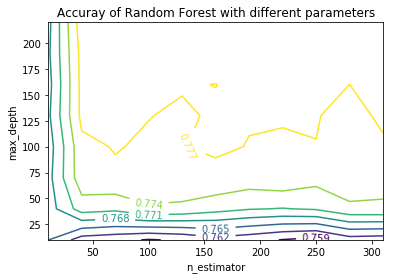
\includegraphics[width=10cm]{random_forest.png}
    \caption{Accuracy of random forest with different parameters.}
    \label{rf}
    \end{figure}
    
    \item \textbf{Adaboost:} Adaptive Boosting algorithm is a kind of boosting algorithm for classification problem that iteratively trains weak classifiers (e.g. decision trees) on re-weighted training set. Each time the weights of misclassified data points are adjusted such that later classifiers can more focus on hard cases. Hence, AdaBoost can effectively reduce bias of simple base models. AdaBoost is already included in SKlearn, so we can implement it by comparing and tuning relevant parameters, including n_estimators, and learning_rate.
    \begin{itemize}
    \item \textbf{n_estimators:} We tested the accuracy of AdaBoost with different number of estimators as Figure \ref{ada} shows. From the figure we can see that the optimal performance was achieved at approximately 200 estimators.
    \item \textbf{learning_rate:} We tried various learning rates and found that with learning_rate = 1 optimal performance is attained.
    \end{itemize}
    
    \begin{figure}[H]                          
    \centering
    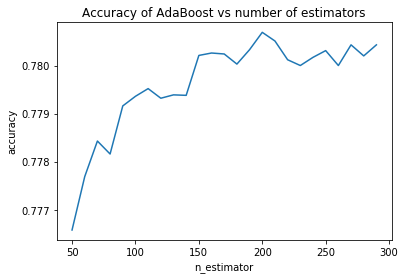
\includegraphics[width=10cm]{AdaBoost.png}
    \caption{Accuracy of AdaBoost using different number of estimators.}
    \label{ada}
    \end{figure}
    
    \item \textbf{XGboost:} XGBoost is short for “Extreme Gradient Boosting”, where the term “Gradient Boosting” is proposed in the paper Greedy Function Approximation: A Gradient Boosting Machine, by Friedman. XGBoost is based on this original model. The parameters are the undetermined part that we need to learn from data. XGBoost is not contained in SKlearn package, so we need to install package first and then test the model with different parameters including max_depth, learning_rate and n_estinators.
    
    \begin{itemize}
    \item \textbf{0:} We tested the accuracy of XGBoost with different number of estimators as Figure shows. From test result we can see that when number of estimators is in range of 200 to 300, the model performances well. And from the figure we can see that the optimal performance was achieved at approximately 240 estimators when learning rate is 0.1.
    \item \textbf{learning_rate:} We tried various learning rates and the optimal performance is achieved when learning rate = 0.1. When we increased this learning rate, the accuracy had significant reduction.
    \item \textbf{max_depth:} Max depth is another parameter that has great impact on performance.This parameter determines when to stop the training process and a reasonable value could avoid over-fitting. Based on cross validation test result, max_dept = 10 is optimal choice for us to balance accuracy and over-fitting
    \end{itemize}
   
    \begin{figure}[H]                           
    \centering
    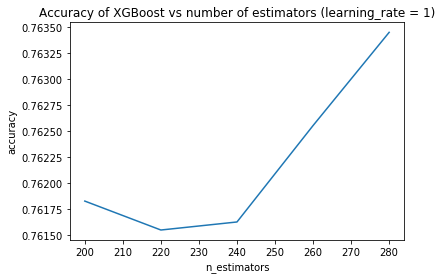
\includegraphics[width=10cm]{XGBoost_lr=1.png}
    \caption{Accuracy of XGBoost with different number of estimators at learning_rate = 1.}
    \label{xg}
    \end{figure}
    
    \begin{figure}[H]                           
    \centering
    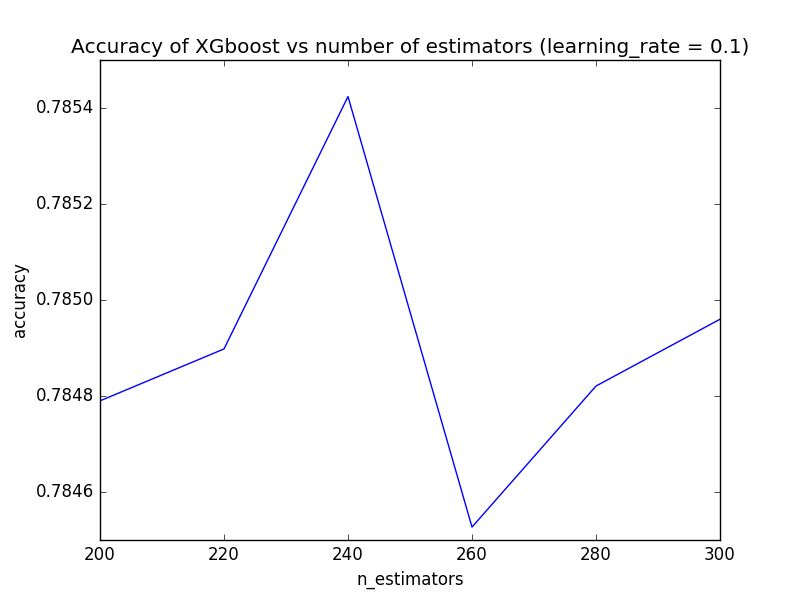
\includegraphics[width=10cm]{XGBoost_lr=0.png}
    \caption{Accuracy of XGBoost with different number of estimators at learning_rate = 0.1.}
    \label{xg0.1}
    \end{figure}
    

    \item \textbf{XGboost and Adaboost:} Based on the results of comparison of different models, we choose two models (XGboost and asaboost) that performance best among those models, and tried to combine those two models to improve the performance. The parameters for XGboost are max_depth=10, learning_rate=0.1, n_estimators=240, and the parameter for adaboost is n_estimators = 200.

    The approach for the combination of two models is that we multiplied a coefficient to the output of each model, and the sum of two coefficient equals to 1, then we add the two output together and set up a random number with uniform distribution on [1, 2], if the added output is bigger than the random number, set the output to be 2 and if the output is smaller than the random number, we set the output to be 1. 

    In this way, for the output for the both model is the same, we would choose this output, but if the output is not the same i.e. one output is 1 and the other is 2, then the final output depends on the comparison with the random number. For the model multiplied with larger coefficient, the final result is more likely to be the same as the result of this model. So in this model that combined with two models, the multiplied coefficient to the output will affect the prediction accuracy. Here follows a plot that shows the relationship between proportion of two models and the cross-validation accuracy.

    Specifically, we calculate the output with y0 = y(XGboost)*a + y(adaboost)*(1 - a), and then compare y0 with the random number to obtain y = 1 or y = 2.
    
     \begin{figure}[H]                           
    \centering
    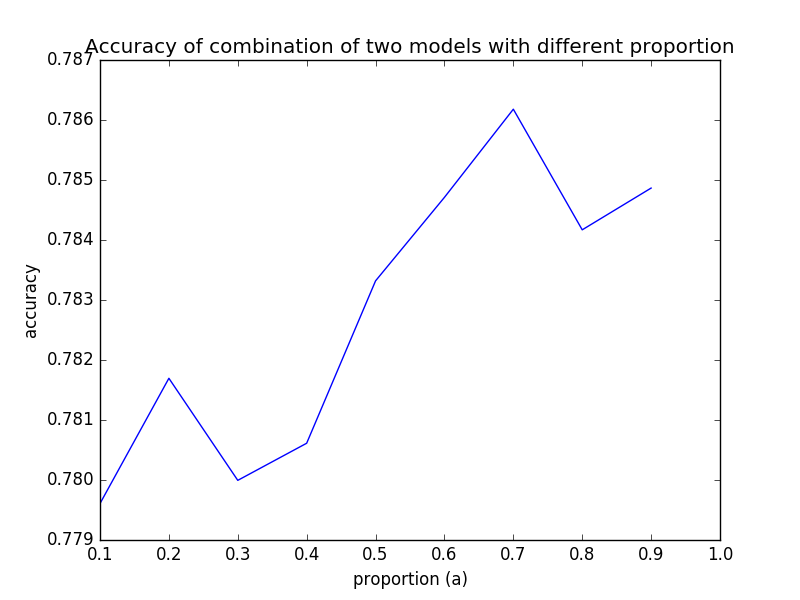
\includegraphics[width=10cm]{combine.png}
    \caption{Accuracy of combination of two models with different proportion.}
    \label{com}
    \end{figure}
    We can see from Figure \ref{com} that when a = 0.7, the model performances best, so we chose this as our final model.

    \end{itemize}

\end{itemize}



\section{Model Selection}
\medskip
\begin{itemize}

    \item \boldline{Scoring} \\
    % Insert text here.
    First, among the models that we have learned, we take off logistic regression and SVM, because they are too simple models for such a task with some many dimensions of input. And we then run a test on five other models: "Nearest Neighbors", "Decision Tree", "Random Forest", "Neural Net", "AdaBoost". 
    
    \begin{figure}                           
    \centering
    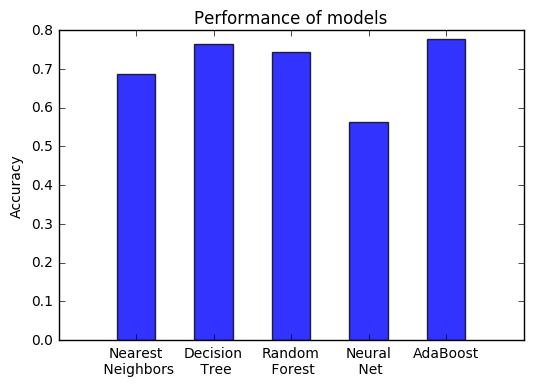
\includegraphics[width=10cm]{performanceOFmodels.png}
    \caption{Cross-Validation score of five models.}
    \label{perOFmodel}
    \end{figure}

    \item \boldline{Validation and Test} \\
    % Insert text here.
    We use 5-fold cross-validation to measure the performance of each model. From the result above Figure \ref{perOFmodel}, random-forest, and Adaboost have better scores. So we choose to optimize this two methods. And since ada-boosting perform slightly better than random-forest, we think boosting works better than bagging so our dataset has high bias and small variance so we then introduced XGboost for further bias reduction.

\end{itemize}



\section{Conclusion}
\medskip
\begin{itemize}

    \item \boldline{Discoveries} \\
    % Insert text here.
    In this particular project, we found that for this particular kaggle project, boosting works better than bagging. In the end, we chose to use a blend of gradient boost and adaboost. By doing so, we acchieved a pretty good rank on testdata2008. However, since boosting reduces bias but increases variance, our performance on 2012 data is not so good maybe because of high variance.
    \item \boldline{Challenges} \\
    % Insert text here.
    The most challenging part is computational power. The computations really take a lot of time that we have to keep our laptops working at night. But we still could have increase our performance if there's more time for running tests.
    \item \boldline{Concluding Remarks} \\
    % Insert text here.
    In this mini-project, we learned how to from the very start, picking models, then optimized parameters and in the end report final values and write reports -- a complete process of working on a machine learning task. After participating in this kaggle competition, we now have better understanding about both datasets, models, testing and optimization. We appreciate the chance of competing with our classmates and we are looking forward to working on more challenging course projects in the future.
\end{itemize}



\end{document}
